%File: formatting-instruction.tex
\documentclass[letterpaper]{article}
\usepackage{aaai}
\usepackage{times}
\usepackage{helvet}
\usepackage{algorithm}
\usepackage{algpseudocode}
\usepackage{courier}
\usepackage{graphicx}
\graphicspath{{./figure/}}
\frenchspacing
\setlength{\pdfpagewidth}{8.5in}
\setlength{\pdfpageheight}{11in}
\pdfinfo{
/Title (Multiple Object Tracking using Spatial Reasoning)
/Author (Xiaoyu Ge, Jochen Renz)}
\title{Multiple Object Tracking using Spatial Reasoning}
\author{Xiaoyu Ge \and Jochen Renz \\
Research School of Computer Science\\
The Australian National University \\
Canberra, Australia\\
\{xiaoyu.ge, jochen.renz\}@anu.edu.au
}
\setcounter{secnumdepth}{0}  
 \begin{document}
\maketitle    
\begin{abstract}
Intelligent agents perceive the world mainly through images captured at  different time points. Being able to track objects from one image to another is fundamental for understanding the changes of the world. 
Humans can perform efficient object tracking by common sense reasoning. For example, we know that a free falling object will not change its downwards movement unless acted upon by another force. Given an initial image with a free falling object, we will first check the objects which are below the initial object location in order to find the corresponding object in subsequent images. 

Object tracking has been extensively studied within the context of computer vision. However, reasoning is typically not used to solve this problem. Most tracking algorithms represent and track objects by their visual features and trajectories. Those algorithms become error prone when there are multiple objects with the same appearance that follow similar trajectories, that change trajectories, or when trajectories are not available. 

%In this paper, we propose a solution to the problem of tracking multiple objects across images taken at different time points. We represent objects using general solid rectangles, i.e., rectangles that can have any angle and are not penetrable (GSRs). GSRs are often used in computer vision and video games. We present a modified version of the GR-n representation [Ge and Renz, IJCAI 2013] that allows us to specify useful spatial constraints and infer possible spatial changes of GSRs. 

Our solution is closer to human reasoning in that it considers spatial relations and physical properties of objects. It can improve tracking accuracy significantly by qualitatively predicting possible motions of objects and discarding matches that violate spatial constraints. 

We evaluate the solution in a real video gaming scenario. We capture sequences of screenshots of the game where multiple objects are moving, and compare the tracking accuracy by varying the length of the intervals between the time points at which the screenshots are taken. Our solution is flexible enough that can be extended with more powerful qualitative reasoning models to tackle multiple object tracking when the time interval between images is long. 
\end{abstract}
\section{Introduction}

Visual perception is one of the main sources of information about the world. Most intelligent agents have eyes, cameras, or other optical devices to "see" their environment and to detect changes in their environment. The information these devices provide is in the form of image sequences, or if the image sampling rate is high enough, we call it video.
Image understanding \cite{sonka1999image,sridhar2011video} and object detection \cite{papageorgiou1998general} are essential methods for extracting useful information from images. Equally essential is object tracking \cite{yilmaz2006object}, that is the ability to identify the same object in a series of images or in video and to track its movement and its changes. Existing object tracking methods typically rely on the visual appearance of objects and on their trajectories to successfully track even temporarily occluded objects \cite{yilmaz2004contour,cutler2000robust,viola2005detecting}.
Similar methods are used for multiple object tracking \cite{berclaz2011multiple,yang2005fast,han2004algorithm}. 

In this paper we are interested in a problem that can occur when intelligent agents observe the world through visual perception and have to track changes.
It can be described as follows: Given two images, let's call them "before" and after", that depict the same scene at different times. Between the two images, certain physical actions have been happening that affected the locations and possibly the states of the objects in the scene. Our task is to find a match between the objects in the "before" image with the objects in the "after" image that is consistent with the effects of the physical actions that happened between the two images. In case there are multiple consistent matches, we want to identify the most plausible one.

It is clear that this problem is relatively straightforward to solve if the visual appearance of all objects in each image is unique, as we simply match the objects that have the same visual appearance. The problem gets challenging, if multiple objects have the same visual appearance. We say that objects of the same visual appearance have the same type and we can only match objects of the same type. Whenever there are multiple objects of the same type, existing object tracking methods are not applicable any more, as we have to deal with a combinatorial number of possible matches that depend on non-visual cues. 

There are different variants of this problem depending on the way the relevant physical actions are specified or unspecified. In general, the actions pose additional constraints that have to be satisfied. These constraints can vary from case to case and typically depend on the application. One variant of the problem is when the specific actions that are responsible for the changes are unknown. 
Then the task is to find a match that are consistent with actions we do not even know. 
We could also formulate the problem as identifying physical actions that explain a proposed match.
Depending on the speed of the changes, it is clear that the longer the time gap between the "before" and the "after" image, the less accurate a match might be.

There are many real-world situations where this problem occurs. For example in natural disasters such as earthquakes, storms, or tsunamis, where we often see before and after images, also in terrorist attacks or bomb explosions. But there are also less dramatic situations, for example a satellite that takes another image of the same site at the next fly-over, or a stationary webcam that sends images only at certain time intervals. 

Our interest in this problem is motivated by the Angry Birds AI competition \cite{abCompetition} where the task is to build an AI agent that can play Angry Birds as good as the best human players. One major problem in this context is to be able to accurately predict the outcome of an action. To do this, we need to learn from previous cases where the effect an action had on a given scenario is known. As input to the machine learning algorithms that are supposed to learn the outcome of actions, we need to know the initial scenario, the action that was used and the effect the action had on each object in the initial scenario. Thus, we need to know exactly which object in the initial state corresponds to which object in the resulting state. In order to be able to learn a huge number of cases, we need to be able to automate the matching between objects in the "before" and in the "after" image.

We evaluate our proposed solution using the Angry Birds scenario. We take subsequent screenshots of an active Angry Birds game taken with varying time gaps and apply our method to match the objects between successive screenshots. We measure the accuracy of our method by using the percentage of correct matches out of the total number of possible mismatches. As expected, it turns out that the smaller the time gaps, the higher the accuracy of the matches. But overall the quality of our mathces is very high. 



\section{Detection and Representation of Objects in Images}

In order to be able to track objects in images, we obviously have to be able to first obtain objects from images. Object recognition \cite{belongie2002shape,lowe1999object} is one of the hardest and most researched problems in Computer Science and it is still unsolved in its generality. In this paper we assume that objects can be detected and we will use cases where object detection is solved and works. In particular, we use images taken from the Angry Birds game, as this is the main motivation of our work in this paper. 
The basic software provided by the Angry Birds AI competition organisers includes an object recognition module that detects all known objects with reasonable accuracy and places a minimum bounding rectangle (MBR) around them. In this paper we use an advanced version of the object recognition module which is based on a student project by Andrew Wang and which will be integrated to the basic software soon \cite{andrewwang}. This software detects the real shapes of all known objects plus the contour of the ground. For our paper, we only consider rectangular objects and circular objects. We use an MBR to approximate the region occupied by a circle and use exact shapes for the general solid rectangles (GSR), i.e. rectangles that can have any angle and are impenetrable, as is the case in Angry Birds. 

In order to represent these objects we use a qualitative spatial representation in addition to the real shape and location of the objects. 
% 
%"Our method is based on qualitative spatial calculi and reasoning techniques developed in the qualitative spatial reasoning (QSR) community."
%
%We focus on rectangles and circles only.
%\section{Objects Representation with the extended GSR-n (EGSR)} 
%
%We use a minimum bounding rectangle (MBR) to approximate the region occupied by a circle and use exact shapes for the general solid rectangles (GSR), i.e. rectangles that can have any angle and impenetrable. 
%
Many rectangle-based qualitative spatial calculi \cite{balbiani1998model,cohn2012thinking,sokeh2013efficient} have developed in the context of Qualitative Spatial Reasoning \cite{cohn2008qualitative}. These calculi typically deal with one or more spatial aspects such as topology, size, direction, or distance, and make a number of qualitative distinctions according to these aspects. There is currently only one spatial calculus that specifically deals with rectangles of arbitrary angles, the GSR-n calculus proposed by \cite{Ge2013}. GSR-n is a comprehensive spatial representation of GSRs. It defines eight contact sectors that correspond to the eight edges and corners of the rectangles. As shown in Figure~\ref{GSR}(a) and (b), we distinguish eight sectors for regular rectangles ($R_1,\ldots,R_8$) and eight sectors for angular rectangles ($A_1,\ldots,A_8$). Given two GSRs $o_1$ and $o_2$ that contact each other via $sector_1, sector_2 \in \{A_1, ..., A_8, R_1, ..., R_8\}$, the contact relation between $o_1$ and $o_2$ can be expressed as the constraint $o_1 \, (sector_1, sector_2) \, o_2$ (Figure \ref{GSR}.c). With the contact relations, GSR-n allows us to distinguish if and how two objects contact each other. Since the objects can only interact via contacts, we can further infer the possible motions of an object from the GSR relations the object holds with others. GSR-n also defines a set $n$ of unary relations using  $Qualitative\,Corner\,Instantiations$, which qualitatively describes the size and leaning direction of a GSR. Since we represent the rectangles using their real shapes, we do not need the unary relations. 
\begin{figure}[h!]
\centering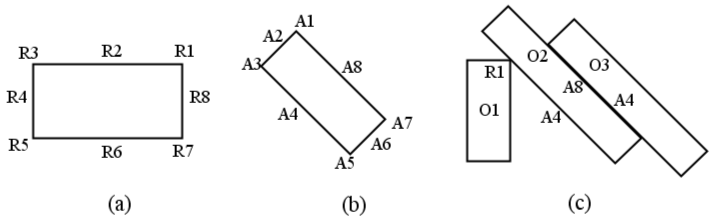
\includegraphics[scale=0.25]{GSR.png}\caption{Contact sectors of (a) a normal rectangle (without rotation) and (b) an angular rectangle. (c) An example scenario where $o_1 (R_1, A_4) o_2$, $o_2 (A_8, A_4) o_3$}
\label{GSR}
\end{figure}

\subsection{Objects Representation with the extended GSR-n relations (EGSR)}

Given two GSRs, we obtain the contact relation by enumerating all the plausible combinations of the two GSRs' contact sectors and for each combination calculating the distance between the two sectors. The combination with the shortest distance constitutes the contact relation. Note, the shortest distance can be non-zero. A non-zero distance means the two GSRs are separate, otherwise touch. So unlike the original definition that the contact relation can only be assigned when two GSRs touch, here we can assign a contact relation for any pair of GSRs. To distinguish whether two GSRs touch or not, we turn to qualitative distance relations which are covered in the next section.
\begin{figure}[h!]
\centering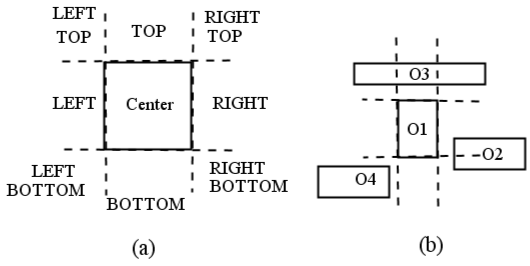
\includegraphics[scale=0.35]{CardinalTiles.png}\caption{(a) The nine cardinal tiles (b) An example scenario where $o_3 (TOP) o_1$, $o_2 (RIGHT) o_1$, and $o_4 (BOTTOM\,LEFT) o_1$}
\label{CardinalTile}
\end{figure}
The problem with GSR-n is that it uses $(\emptyset, \emptyset)$ to represent the spatial relation between all the non-touched GSRs. Thus, it introduces ambiguities when the rectangles are disconnected. To overcome the ambiguities, we extend the original GSR-n by integrating it with the cardinal tiles \cite{goyal1997direction}. Specifically, we partition the embedding space around an reference object into nine mutually exclusive tiles(see Figure \ref{CardinalTile}.a). The centre tile corresponds to the minimum bounding rectangle of the object and the other eight tiles correspond to the eight cardinal directions. We call the $LEFT$, $RIGHT$, $BOTTOM$, $TOP$ core tiles.  

\begin{figure}[h!]
\centering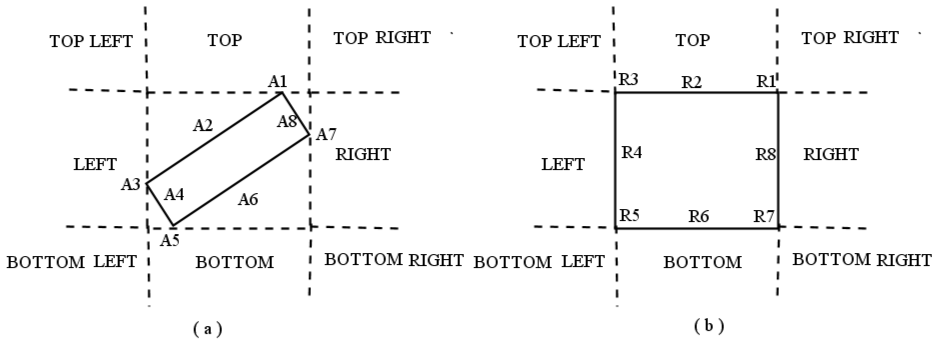
\includegraphics[scale=0.25]{EGSR-relations.png}\caption{Contact sectors and Cardinal directions of (a) an angular rectangle and (b) a normal rectangle}
\label{EGSR}
\end{figure}
The new representation is called EGSR (see Figure \ref{EGSR}). Given a set ${\cal B}_{GSR}$ of GSR contact relations and a set ${\cal B}_{card}$ of cardinal tiles,  we add $\bot$ to both sets to indicate a unassigned relation, an EGSR relation is then written as $(r_1, r_2), r_1 \in {\cal B}_{GSR}\cup \{\bot\}, r_2 \in {\cal B}_{card}\cup \{\bot\}$. We abbreviate $(r_1,r_2)$ by the cardinal tile $r_2$ or by the contact relation $r_1$ if it is clear which one is meant. 

We compute the EGSR relation between two spatial objects by first checking whether their MBRs intersect or boundary touch. If so, we assign a GSR-n relation accordingly. Otherwise, one of the eight cardinal tiles will be used. If one object's MBR occupies multiple tiles of the referred object, we will assign the core tile occupied by the MBR (see Figure \ref{CardinalTile}.b). Note, when one object's MBR occupies more than one core tiles of the referred object, it must intersect or boundary touch the referred object's MBR, in this case, GSR-n relation will be assigned instead. All EGSR relations are obviously converse, e.g. the converse of $TOP\,LEFT$ is $BOTTOM\,RIGHT$, the converse of $(R_4, S_7)$ is $(S_7,R_4$).

\cite{wallgrun2010qualitative} introduced the notion of qualitative interpretation that extracts qualitative descriptions from the input data. A scenario containing multiple spatial objects can be qualitatively interpreted by EGSR via a qualitative constraint network (QCN). QCN is a labelled graph where each node corresponds to an object and directed edges represents relational constraint that has to hold between the two objects. 
Figure \ref{QCN} shows an example of a QCN based on EGSR relations.


 \begin{figure}[h!]
\centering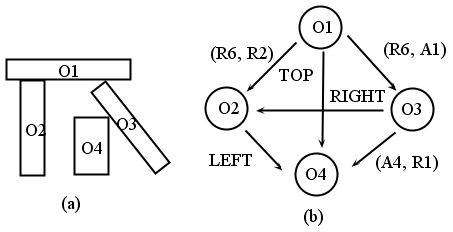
\includegraphics[scale=0.45]{QCN.png}\caption{(a) A spatial scenario where the four rectangles form a stable structure under downward gravity (b) The corresponding qualitative constraint network}
\label{QCN}
\end{figure}

\section{Efficient Matching by Approximating Movement}\label{approxM}

The search space of the matching problem is huge as there is a combinatorial number of potential matches between any two object sets. However, most matches can be avoided by searching through the corresponding objects only in a limited area. The area of the initial object should therefore cover all the objects in the subsequent scene that can be potentially matched to the initial object.  We use a circular region to represent this area. The circle's centre is located at the centroid of the initial object and the radius of the circle is the maximum shift of the centroid. The radius is calculated as $v \times t$ where $v$ is the maximum velocity of the object and $t$ is the time gap between the initial and subsequent scenes. This calculation ensures that the circle can adapt to different time gaps. We call this circle the $movement\,bounding\,circle$(MBC).  
\begin{figure}[h!]
\centering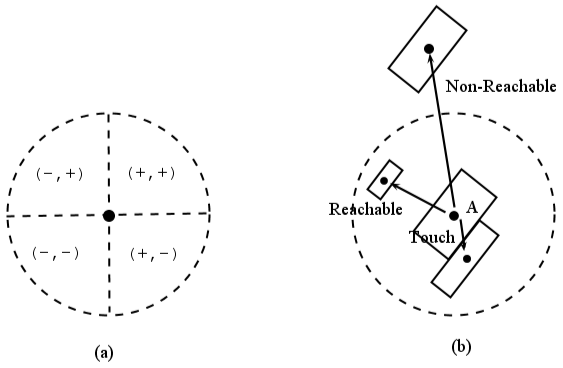
\includegraphics[scale=0.3]{quadrants.png}\caption{(a) The four quadrants of a MBC (b) Qualitative distance with respect to object A and its MBC}
\label{Quadrants}
\end{figure}

The relative distance between two objects can then be allocated to three meaningful classes, namely touch, reachable, and non-reachable (Figure \ref{Quadrants}.b). An object $o$ can touch another object $o^\prime$ at one of its contact sectors. $o^\prime$ is reachable by $o$ if $o^\prime$ is within the MBC of $o$ otherwise non-reachable. 

The MBC can be divided into four quadrants to further restrict the search area. A quadrant of an object is said to be active if the object is likely to be in that quadrant at the next time point, otherwise the quadrant is inactive. The search space can be reduced by first searching possible matches in the active quadrants, if there are no such matches, then searching in the other quadrants. Given a MBC $C$, the active quadrants are $C^{(i,j)}, i,j \in \{-, +, *\}$ where $(+,+)$, $(+,-)$, $(-,-)$, $(-,+)$ correspond to the top-right, top-left, bottom-left, bottom-right quadrants respectively (Figure \ref{Quadrants}.a). $(*, *)$ refers to an arbitrary quadrant. 

We can infer the active quadrants for an object by approximating the movement direction of the object, i.e. by estimating which of the quadrants the object is most likely to be in at the next time point. Object movement can be inferred from impact. Knowing the direction and the force of an impact, one can approximate the subsequent movements of the objects affected by the impact, directly or indirectly. When the impact information is not available, we can still approximate the movement by analysing structural properties, e.g. the stability of an object or a group of objects. An object is stable when it is supported and remains static. %An unstable object can have one of two possible motions, free fall if it is unsupported or fall to the side where there are no supports. %

We call the movement approximating problem we want to solve MQSR($\Theta$, \cal{R}, $M_{\cal{R}}$) where $\Theta$ is a set of objects in a spatial scenario and \cal{R} is a qualitative spatial representation of the objects. $M_{\cal{R}}$ is a reasoning model composed of a set of configurations written in the relations defined by \cal{R} by satisfying which the corresponding active quadrants of an object can be obtained. For each object in $\Theta$, we want to estimate the object's active quadrants by evaluating the object's spatial configurations against $M_{\cal{R}}$.

\cite{Ge2013} defined four kinds of supports that can make a solid rectangle stable and provided the corresponding GSR configurations. Our model $M_{\cal R}$ contains all such stable configurations. Given each object, the model will evaluate the stability of the object by the configurations and return $C^{(*,-)}$ for the unstable objects.

We solve the problem in the Angry Birds scenario where a bird hit usually comes from the left. We use $EGSR$ to represent the spatial configuration of a scenario. The model we use is mainly based on the stability analysis.


A stable object may become unstable if it loses a support due to a bird hit. From the bird's trajectory, we can determine which object will be hit by the bird, and approximate the stability of the resulting scenario with the removal of that object (Figure \ref{BirdImpact}). 

We can get a more restricted area, $C^{(+,-)}$ or $C^{(-,-)}$, by analysing the direction in which the object is falling. For example, a right / left leaning rectangle will fall to the right / left if there is no support at the right / left side, and the corresponding active quadrant is $C^{(+,-)}$ / $C^{(-, +)}$ (Figure \ref{QudrantsEstimation}). Here we illustrate how can we express the configurations described in the example using EGSR relations. We denote the left leaning and right leaning objects as $O^L$, $O^R$ respectively, and the MBC of an object $o$ is written as $C_{o}$. The two configuration can be expressed using EGSR relations:
\begin{enumerate}
\item Right-leaning: $\forall o^R_1\,:\, \exists o^*_2\,o^R_1 (A_5, *) o^*_2 \wedge\neg\exists o^*_3\,o^R_1 (A_6, *) o^*_3 \wedge\neg\exists o^*_4\,o^R_1 (A_7, *) o^*_4 \Rightarrow \, C_{o^A_1}^{(+,-)}$

\item Left-leaning: $\forall o^L_1\,:\, \exists o^*_2\,o^L_1 (A_5, *) o^*_2 \wedge\neg\exists o^*_3\,o^L_1 (A_3, *) o^*_3 \wedge\neg\exists o^*_4\,o^L_1 (A_4, *) o^*_4 \Rightarrow \, C_{o^L_1}^{(+,-)}$
\end{enumerate}
The model $M_{\cal{R}}$ contains all such configurations and can be replaced with any other model using $EGSR$ relations. Figure \ref{ScenarioByRules} shows some example scenarios and the corresponding quadrants estimated by $M_{\cal{R}}$

 We will show the model $M_{\cal{R}}$, although simple, is sufficient to solve the tracking problem in the evaluation part.  


\begin{figure}[h!]
\centering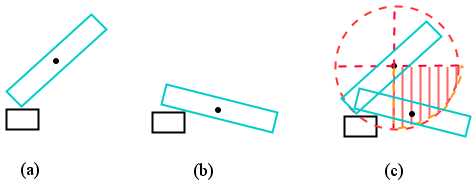
\includegraphics[scale=0.35]{QudrantsEstimation.png}\caption{(a) The right-leaning object (in cyan)  (b) a subsequent scene where the object falls to the right (c) The estimated active quadrant (shadowed area)}
\label{QudrantsEstimation}
\end{figure}


\begin{figure}[h!]
\centering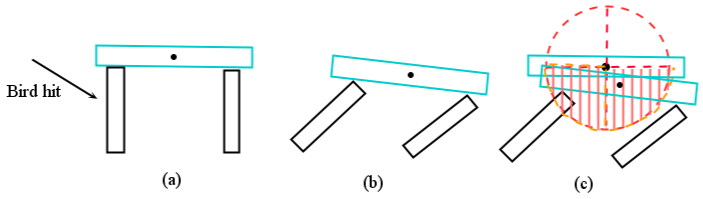
\includegraphics[scale=0.35]{BirdImpact.png}\caption{(a) The object in cyan is stable, and the impending impact is indicated by the arrow (b) A subsequent scene after the bird hit (c) The estimated active quadrant (shadowed area)}
\label{BirdImpact}
\end{figure}

\begin{figure}[h!]
\centering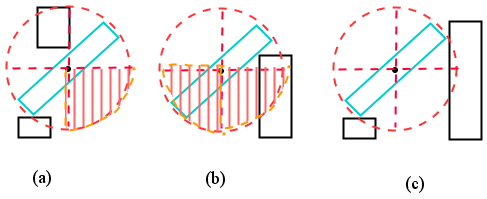
\includegraphics[scale=0.35]{ScenarioByRules.png}\caption{ The active quadrants of $o_1$ is (a)  $C^{(+,-)}$ by satisfying the Right-leaning configuration (b) $C^{(*,-)}$ because there is no object contacts $A_5$ of $o_1$ (c) No active quadrants as the object is stable}
\label{ScenarioByRules}
\end{figure}

\section{Handling Common Movement by Spatial Reasoning}
\label{CM}

One challenge is to determine a match between identical objects that are close to each other and have similar trajectories.  

Figure \ref{SCOExample_2}.a  shows a scene where objects A and B form a slope and three identical squares, $o_1$, $o_2$ and $o_3$, are lying on the slope. Figure \ref{SCOExample_2}.b is a subsequent image where the three squares have rolled down slightly. There are 6 ways in total to match the squares in the two images but only $\{o_1 \sim o_4, o_2 \sim o_5, o_3 \sim o_6\}$ is possible ($\sim$ is a operator that matches one object to another). Because they do not use reasoning about the spatial relations between the squares, some optimization algorithms, e.g.\ minimizing centroid shift, will tend to match $o_2$ with $o_6$. In many cases, object dynamics, such as velocities, are unavailable, thus many of the state-of-the-art tracking algorithms will not work well because of the lack of a suitable dynamic model. 

Humans can solve this case efficiently using spatial reasoning. Since we know the objects are moving at a similar velocity, the relative spatial changes among them are subtle. Hence the spatial relations between those objects are unlikely to become converse while they are moving. When matching, we try to keep the original spatial relations among the subsequent objects. 

We emulate this reasoning in testing a match by first identifying those objects that are following a similar trajectory and then determining whether any relation has become converse in the subsequent image. 

Objects are likely to follow a common trajectory if they are all in contact with some other objects and the contact relations are the same. The objects may be influenced in the same way since their interactions are through the contacts with the other objects. We say that such objects form a \emph{spatially correlated object} (SCO). Figure \ref{SCOExample} shows some examples of SCOs in a typical Angry Birds scenario.

Given a set of initial objects, we obtain the SCOs by checking the node equivalence in the corresponding EGSR network. A node is equivalent to another if the two nodes have the same contact relations with other nodes. Thus the slope example has only one SCO: $\{o_1, o_2, o_3\}$ (see Figure \ref{SCOExample_2}.c).

Having identified an SCO, we then check the spatial relations between the matched objects in the subsequent image. Formally, let $R$ be a set of EGSR relations. The converse of a relation $r \in R$ is written as $r^{\prime} \in R$. Given a group objects that form a spatially correlated object in the initial image $O = \{o_1, o_2, ... , o_k\}$ and a set of subsequent objects $O^\prime = \{o^{\prime}_1, o^{\prime}_2, ..., o^{\prime}_k \}$ with a match, $\forall i\leq k, o_i \sim o^{\prime}_i$, between them, the spatial constraints can be written as $\forall o_i,o_j\in O, \exists r\in R$ such that $o_i \{r\} o_j \Rightarrow o^{\prime}_i \{r^{\prime}\} o^{\prime}_j$ \emph{does not hold}, for $i,j \leq k$. If a match violates the constraints, we will try all the other possible matches for the SCO until the violation is resolved. If all matches violates the constraints, we keep the original match.  

In the slope example, the match $\{o_1\sim o_4, o_3\sim o_5, o_2 \sim o_6\}$ violates the constraint because $o_2\{LEFT\}o_3$ and $o_6\{RIGHT\}o_5$ where $RIGHT$ is the converse of $LEFT$.

\begin{figure}[h!]
\centering\includegraphics[scale=0.7]{SCOScenario.png}\caption{(a) A typical Angry Birds scenario (b) SCOs (each highlighted by a different color)}
\label{SCOExample}
\end{figure}

\begin{figure}[h!]
\centering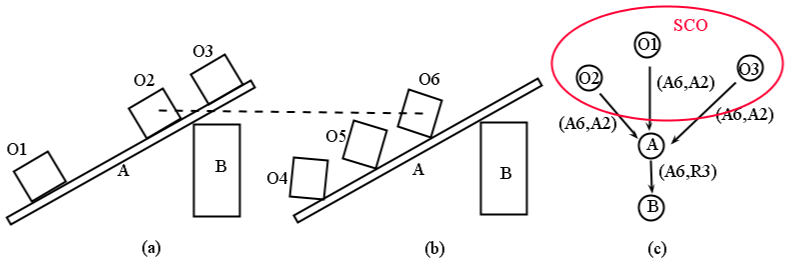
\includegraphics[scale=0.3]{SpatiallyCorrelatdScenario.png}\caption{(a) An initial scene (b) A subsequent scene where the squares have rolled down slightly (c) The EGSR constraint network of the initial scene (only retain the edges indicating contacts) and the SCO}
\label{SCOExample_2}
\end{figure}


\section{A Method for Tracking Objects}

We proposed a method that utilizes all the above mentioned techniques to solve the matching problem (see Alg. \ref{algo}).

Let $O$ and $O^{\prime}$ be a set of objects in an initial image and a subsequent image taken at a later time, respectively. For ease of notation, we will refer to objects in $O$ as initial objects and objects in $O^{\prime}$ as subsequent objects.

First, the method randomly assigns a unique ID to each initial object, and estimates the MBC quadrants for each object according to the object's spatial relations (see Alg. \ref{algo} line \ref{MA}). The list of possible matches for each initial object is set so that it contains only the subsequent objects that are of the same type and within the MBC quadrants (see Alg. \ref{algo} line \ref{SetPossible}). The method then creates a preference list from the possible matches of each of the initial objects: the subsequent objects in the preference list are sorted by the size of the centroid shift from the initial object in ascending order. The method matches the two sets of objects using a stable marriage algorithm \cite{gale1962college} with the pre-computed preference lists (see Alg. \ref{algo} line \ref{calPref}). The algorithm ensures each match is stable in the sense that no pair of objects would prefer each other over their matched partners. 

Then, the method finds all groups of spatially correlated objects from the initial objects and gets their corresponding objects from the match (see Alg. \ref{algo} line \ref{getSCO}). The method then checks to see whether the spatial constraint  has been violated. If it has, it resolves this accordingly (see Alg. \ref{algo} line \ref{CommonMotion}).

\section{Implementation}
We implemented our method and applied it to the Angry Birds where the vision system can detect the exact shapes of the objects \cite{andrewwang}. The objects' visual appearance are restricted to a finite number of templates (see Figure \ref{Templates}).  
\begin{figure}[t!]
\centering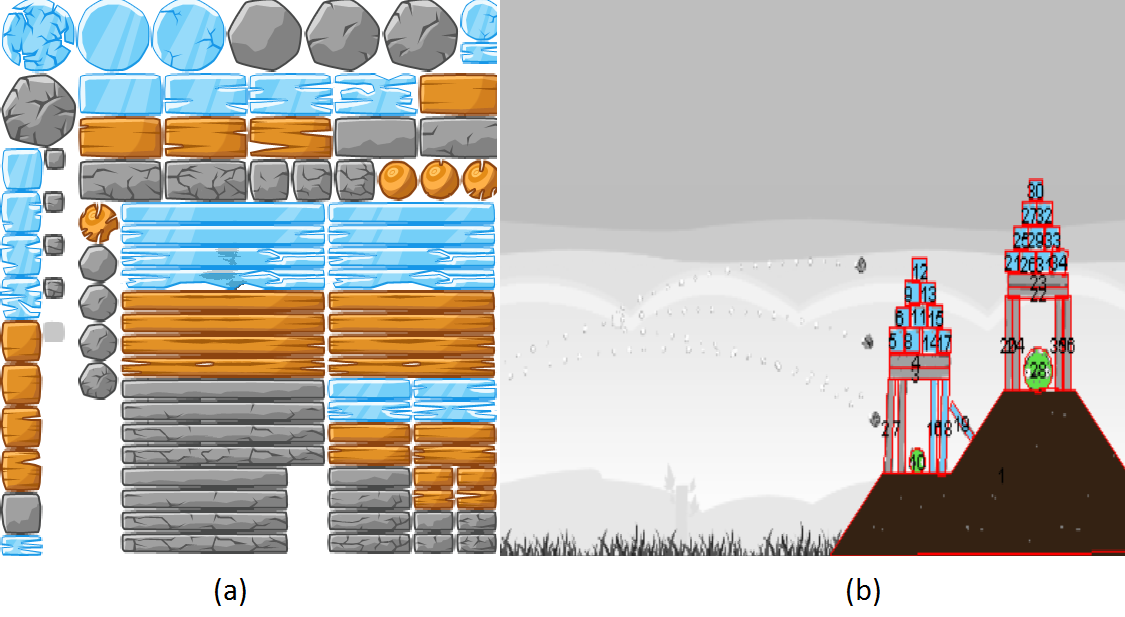
\includegraphics[scale=0.28]{Templates.png}\caption{(a) Main Templates used in Angry Birds (b) The vision detects the real shapes of the objects in a typical Angry Birds scenario}
\label{Templates}
\end{figure}
The vision system has the following limitations that can severely affect the matching accuracy: 
\begin{itemize}
\item Misdetection of damaged objects. Damaged objects will be detected as a number of separate smaller pieces. (Figure \ref{Fragments}.b) 
\item Debris is not recognized so that the system cannot determine whether an object, say a stone, is a real stone or just a piece of debris from a previously destroyed stone (Figure \ref{Fragments}.a).
\item Occlusion of objects is not handled. Objects can be partially or entirely occluded by debris or other game effects e.g. scores or clouds around the hit point (Figure \ref{Fragments}.c)
\end{itemize}
\begin{figure}[t!]
\centering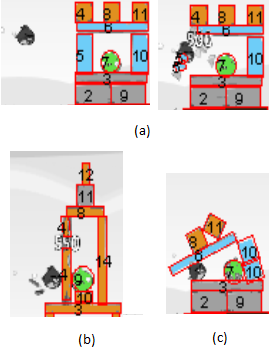
\includegraphics[scale=0.7]{Fragmentation.png}\caption{(a) The object with ID 5 is broken into pieces by a hit (b) The object with ID 4 is partially occluded (c) The object with ID 10 is damaged and detected as two separate blocks}
\label{Fragments}
\end{figure}

The fragmentation of objects creates new objects in subsequent images and the new objects are not directly related to the initial ones. The varying number of objects from one scenario to another can introduce ambiguities which can confuse the tracking algorithm. 

There are several approaches for tackling this problem.\cite{Occlusion1,Occlusion2,Occlusion3}. Most of them largely depends on their underlying tacking algorithms and their own ad-hoc occlusion reasoning models e.g. inference graph, Bayesian network. 

We create an approach that can effectively deal with the fragmentation in the Angry Birds context where objects are created on a finite number of templates. 
Identifying which objects have been destroyed is also important, we show our method can determine this as well in the following section.   

\subsection{Handling Fragmentation and Occlusion}
 
In Angry Birds, fragmentation is mainly due to the destruction of objects, partially occlusion, and damage. By recognizing these fragments, the method is able to infer whether an object has been destroyed, damaged, or occluded, which leads to robust tracking. We achieve this in three steps:

First, we identify all the subsequent objects that could be fragments. Specifically, we classify the initial and subsequent objects by their templates. For each template $T$, there a set $T_{ini}$ of initial objects and a set  $T_{sub}$ of subsequent objects with the same template. We treat all the objects in $T_{sub}$ as potential fragments if $T_{sub}$ contains more objects than $T_{ini}$.

Fragments are then arranged in groups where all the fragments in a group can form one of the templates. The shape formed by the fragments is an oriented minimum bounding rectangle (OMBR) that bounds all the fragments (see Figure \ref{OMBRs}.a). We then treat the OMBR as one object in the subsequent image, so that it can be matched with one of the initial objects.  Once the OMBR is matched, all the fragments from the corresponding group are also matched, i.e. assigned with the same ID. In some rare cases, a fragment may be included in more than one OMBR. So we add an additional constraint that a fragment is not allowed to be common to more than one OMBR.

We label the unmatched fragments as debris. Destruction of an object will create a cluster of debris around the object's location. The pieces of debris can be of any shape, e.g. a circle or polygon and will diffuse until they disappear after 1--3 seconds. Given an object $o$ in the initial scenario, we search for its debris if no subsequent objects can be matched with $o$ (including the OMBRs created from the fragments). We first draw the MBC of $o$. The set of potential fragments are those fragments within the MBC excluding those that have been matched. The set of the objects is labelled as debris of $o$ and $o$ is marked as destroyed (see Figure \ref{OMBRs}.b). In this process, some pieces of debris might be from more than one initial objects and we do not explicitly label pieces of debris with an ID.

An object can also be totally occluded. To deal with this, before the matching, we cache the spatial configurations of all the initial objects. At the end of the matching, we update the cache by replacing each initial object's configuration with the matched subsequent object's so that the cache always maintains the latest configuration of each initial object. If an occluded object recurs in a subsequent image, we match the object by searching through the cache for an unmatched initial object. The occluded object will be matched if it lies in the MBC of that initial object. 
The method determines an object as destroyed if it detects the debris of the object, or when the object has been totally occluded for $n$ seconds. $n$ is tunable and we set $n$ to 1 in the evaluation.  
 
\begin{figure}[t!]
\centering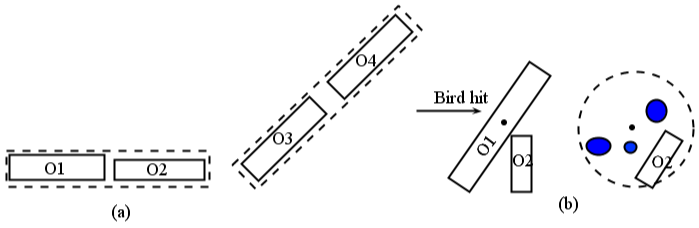
\includegraphics[scale=0.3]{OMBRs.png}\caption{(a) OMBRs are indicated by the dotted rectangles (b) $o_1$ has been destroyed by a bird hit, and the blue dots are recognized as debris}  
\label{OMBRs}
\end{figure}


\section{Evaluation}

Matching an object can be trivial if the object has a unique appearance or the object stays stationary across images. We measure the accuracy of the tracking method by the percentage of correct matches out of the non-trivial mismatches. Specifically, given a set $n$ of objects in an initial scenario and assume $m$ of them are either of unique type or stationary across images, then the total number of possible mismatches is $n - m$. We count the correct matches $c$ of the $n - m$ non-trivial objects. The accuracy is  $c / (n - m)$.

The evaluation has been done in two steps. In the first step, we collect samples from active angry birds scenarios, and obtain the ground truth by applying our method using the smallest time gap. In the second step, we evaluate the method by varying the time gaps and obtain the accuracy by comparing against the ground truth.

 
\subsection{Obtaining Ground Truth}

We collect a sample by capturing a sequence of screenshots before and after a shot using the smallest time gap (50 ms). The average time gap between the beginning and the end screenshot is 10 seconds. That is, a sample contains around 200 screenshots.  We apply our method to the whole sequence so that the method will keep tracking the objects through all of the screenshots, from the first until the last(see Figure \ref{Tracking}). The match between the initial objects in the first screenshot and the subsequent objects in the last screenshot will be saved as the ground truth for later evaluation. We also save the number of stationary and unique objects per sample.

\begin{figure}[h!]
\centering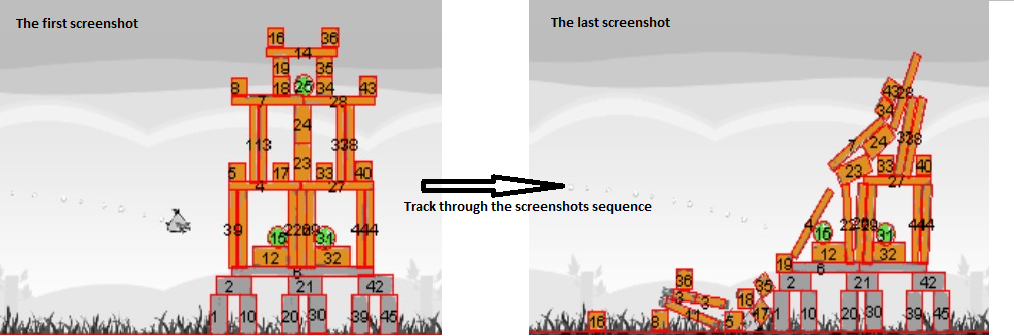
\includegraphics[scale=0.32]{TrackingBackup.png}\caption{The method tracks through the screenshots and label the matched objects with the same ID. The match between the first and last screenshots is saved as the ground truth }
\label{Tracking}
\end{figure}

To automate this process, we run an angry-birds agent that always aims at an random pig on the first 21 poached-eggs Levels \cite{abGame}. The agent starts to capture screenshots once a shot is made, and stops after 10 seconds. At each level, the agent records the screenshots of at most four shots.
We collected 80 samples, and discarded the trivial samples, e.g. when a shot does not affect any object. Finally we have 62 samples. To evaluate the accuracy of the ground truth, we run our method on 10 samples randomly picked from the 62. We determine the accuracy by manually labelling the initial objects and their correspondence in the end screenshot, and compare with the matching. This accuracy is a lower-bound accuracy of matching between a pair of screenshots with the specified time gap, because any incorrect matches made in the intermediate stage will yield mismatches between the first and end screenshots.  

The method can match most of the objects with less than 4 mismatches per sample. The average percentage of the number of correctly matched objects out of the total number of objects is $0.95$. The method achieves real-time performance with average 3 ms per match. To illustrate the significant improvements achieved by the reasoning techniques mentioned above, we compare our method with an approach ($BASIC$) that matches objects using their visual appearance and minimizes the centroid shift between initial and subsequent objects. $BASIC$ is a modified version of our method with the movement approximation, and common movement handling disabled. The results are shown in Table \ref{empiResults}.

\begin{table}[h!]
\caption{Results on the 10 samples(\,$QSR$: the proposed method, $BASIC$: the modified method )}\label{empiResults}
\centering
\begin{tabular}{c|c|c|c|c}
\hline
{} & \multicolumn{2}{c}{Accuracy} & \multicolumn{2}{c}{Mismatch}\\
\hline
Sample & QSR & BASIC & QSR & BASIC\\
\hline
1& 0.91 & 0.5 & 2 & 12\\
2&1.00 & 1.00 & 0 & 0\\
3&0.80 & 0.40 & 2 & 6\\
4&0.85 & 0.54 & 2 & 6\\
5&0.76 & 0.41 & 4 & 10\\
6&1.00 & 0.00 & 0 & 2\\
7&1.00 & 0.56 & 0 & 4\\
8&0.78 & 0.33 & 2 & 6 \\
9&0.71 & 0.42 & 2 & 4\\
10&1 & 0.5 & 0 & 2\\
\hline
\end{tabular}
\end{table}

\subsection{Experimental Results}

We evaluate our method on the 62 samples (12400 screenshots) with varying time gaps, namely 100 ms, 200 ms (the maximum delay in getting screenshot from the server used in Angry Birds AI competition), 300 ms (the time taken by requesting a screenshot plus the vision segmentation), 500ms, and 1000 ms.

For a particular time gap, say 200 ms, the tracking method will start from the first screenshot, go through every $200/50 = 4$ (50 ms is the time gap we use to collect the samples) screenshots of the original sequence, until the last screenshot. E.g. Given a sample with a sequence of screenshots $s_1, s_2, ..., s_{14}$, the method using 200 ms as the time gap will track through $s_1, s_6, s_{10}, s_{14}$ sequentially. The accuracy and mismatches are then obtained by comparing against the saved ground truth. Thus, the mismatches can be viewed as \emph{additional mismatches} to the ground truth. As expected, the accuracy drops down when applying larger time gaps (see Table \ref{empiResults_2}). 

\begin{table}[h!]
\caption{Results on the 62 samples with different time gaps. }\label{empiResults_2}
\centering
\begin{tabular}{c|c|c}
\hline
Time gap (ms) & Average Accuracy & Average Mismatch\\
\hline
100 & 0.85 & 2.22\\
200 & 0.80 & 3.22\\
300 & 0.77 & 3.4\\
500 & 0.70 & 3.98\\
1000 & 0.68 & 4.22\\
\hline
\end{tabular}
\end{table}

\section{Conclusion and Future Work}

We looked at the problem of tracking multiple objects of the same visual appearance across images. Due to the combinatorial number of possible matches between such objects, this problem gets harder the more time passes between images. We developed a method for solving this problem that is based on a qualitative spatial representation of different object properties. We used the Angry Birds game as an example domain, as object detection in this domain is solved for known objects and the number of possible object types is limited. We showed that our method is very accurate in identifying which object in an "after" image correspond to which object in a "before" image, while shooting birds at the structure that protects the pigs. We tested different time gaps between images and analysed how the time gap affects the accuracy of our method. 

Our method should be very useful for the long term goal of building an AI agent that can play Angry Birds better than the best human players. One of the big problems that need to be solved is the prediction of consequences of shots. Our method allows researchers to build sophisticated machine learning algorithms for learning consequences of shots. Instead of just providing a before and after state of shots, we can now automatically identify correspondences between objects in the before and after states, which should lead to much better learning outcomes. As a side-effect it also allows us to identify which objects have been destroyed and which objects haven't. 
It also allows us to test the success and predicted outcome of Angry Birds game playing strategies, such as the structural analysis developed by Peng and Renz \cite{peng13}. 
The time gaps we considered are relevant as they form the minimum time gaps for agents to take and to analyse pictures while actively playing the game. The less often we have to take and analyse screenshots the better. One future goal is to further increase the time gap, but with large time gaps the problem of matching objects is getting extremely hard as there are fewer and fewer cues. We did some initial cognitive studies and asked people to match objects in before and after Angry Birds images. When the time gaps were greater than 2 or 3 seconds, people were mostly unable to find or to explain a correct match. 

As mentioned in the introduction, there are a number of other interesting application domains where similar problems are considered. One problem in other domains might be that object recognition is not as accurate as in the Angry Birds domain, also because the number and type of objects is not restricted. 
One possible line of future work is to extend our method to deal with arbitrary objects and not only rectangular shaped objects. We might be able to use similar methods by using the tightest fitting minimum bounding rectangles that can have any angle around all objects, independent of the objects' shape and orientation.   

\begin{algorithm}[!]
\caption{The Object Tracking Algorithm}\label{algo}
\begin{algorithmic}[1]
\Procedure {MatchObjects}{$objs$}
\State $iniobjs$ \Comment initial objects
%\State $objs \leftarrow$ HandlingFragments($objs$) // add the OMBRs to the objects pool 
\State $solution \leftarrow \{iniobjs, \{\}\}$
\State $pmatches \leftarrow \{iniobjs, \{\}\}$ \Comment possible matches of each initial object
\State $pmatches \leftarrow$ ApproxMovement($iniobjs$, $objs$) \label{SetPossible}
\State CalculatePreference($iniobjs$, $pmatches$)\label{calPref}
\State $freeobjs \leftarrow iniobjs$
\While{$freeobjs$ is not empty}\label{stableMarriage}
\State $iniobj \leftarrow dequeue(freeobjs)$
\State get a next preferred $obj$ from $iniobj$'s preference list  
\If {$obj$ is not assigned yet}
  \State match($iniobj$, $obj$)
  \Else{ $obj$ has been assigned to another initial object $iniobj^{\prime}$}
  \If{$obj$ prefers $iniobj$ to $iniobj^{\prime}$}
  \State match($iniobj$, $obj$), $freeobjs \leftarrow freeobjs \cup \{iniobj^{\prime}\}$
  \Else 
  \State $freeobjs \leftarrow freeobjs \cup \{iniobj\}$
\EndIf 
\EndIf
\EndWhile
\State $cobjsList \leftarrow$ GetSCO($iniobjs$)
\State CommonMotion($cobjsList$,$solution$), $iniobjs \leftarrow objs$
\EndProcedure

\Procedure{GetSCO}{$objs$}\label{getSCO}
\State $cobjsList \leftarrow \{\}$
\For {$obj \in objs$}
\State $cobjs \leftarrow objs$ 
\State $tobjs \leftarrow$ a set of the objects that touch $obj$
\For {$tobj \in tobjs$}
\State $ttobjs \leftarrow$ a set of the objects excluding $obj$ that touch $tobj$ via the same contact relation.
\State $cobjs \leftarrow cobjs \cap ttobjs$
\EndFor
\State $cobjsList \leftarrow cobjsList \cup cobjs$
\EndFor
\Return $cobjsList$
\EndProcedure
\Procedure{ApproxMovement}{$iniobjs$, $objs$}\label{MA}
\For {$iniobj \in iniobjs$}
\State $pobjs \leftarrow \{\}$, compute the active quadrants of $iniobj$, add $obj \in objs$ to $pobjs$ if $obj$ is within the quadrants and have the same type with $iniobj$ 
\State $pmatches \leftarrow pmatches \cup \{iniobj, \{pobjs\}\}$
\EndFor
\Return $pmatches$
\EndProcedure
\Procedure{Match}{$iniobj$, $obj$}
\State $obj.id \leftarrow iniobj.id$, $solution \leftarrow \{iniobj, obj\}$
\EndProcedure
\Procedure{CommonMotion}{$cobjsList$, $solution$}\label{CommonMotion}
\For {$cobjs \in cobjsList$}
\State for each object in $cobjs$, get its matched $obj$ from $solution$. Check whether the spatial constraints are violated. Re-assign until resolved  
\EndFor
\EndProcedure
\end{algorithmic}
\end{algorithm}
\newpage

\bibliography{OT}
\bibliographystyle{aaai}
 \end{document}